\documentclass[8pt]{extarticle}
\usepackage{amsmath}
\usepackage{amssymb}
\usepackage{xcolor}
\usepackage{multicol}
\usepackage{graphicx}
\usepackage{enumitem}
\setlength{\columnsep}{30pt}
\usepackage[T1]{fontenc}
\usepackage{geometry}
\geometry{
    a4paper,
	margin=0.45in,
    includeheadfoot
}
\usepackage{titling}
\setlength{\droptitle}{-7em}
\posttitle{\par\end{center}\vspace{-5em}}
\title{TINF FORMULE}
\author{}
\date{}

\setlength{\parindent}{0pt}
\setlength{\parskip}{0pt}
\setlength{\abovedisplayskip}{2pt}
\setlength{\belowdisplayskip}{2pt}
\setlength{\abovedisplayshortskip}{1pt}
\setlength{\belowdisplayshortskip}{1pt}
\setlength{\multicolsep}{4pt}
\setlist[itemize]{nosep,leftmargin=*}

\newcommand{\infintegral}{\int_{-\infty}^{\infty}}

\begin{document}
\maketitle
\begin{multicols}{2}
	\section*{SIGNALI}
	\[
		E=I(Ri^2(t))=I(\frac{u^2(t)}{R}), \quad P=\lim_{T\to\infty}\frac{1}{T}\int_{-T_0/2}^{T_0/2}Ri^2(t)dt
	\]
	\section*{Periodični signali}
	Fourierov razvoj:
	\[
		x(t)=\sum_{k=-\infty}^{\infty}c_ke^{jk\omega_0t}, \text{ gdje } c_k = \frac{1}{T}\int_{-T_0/2}^{T_0/2}x(t)e^{-jk\omega_0t}dt
	\]
	\subsection*{Snaga}
	\begin{align*}
		P & = \lim_{k \to \infty} \left[ \frac{1}{kT_0} \int_{0}^{kT_0} |x(t)|^2 \, dt \right] \\
		  & = \frac{1}{T_0} \int_{0}^{T_0} |x(t)|^2 \, dt = \sum_{k=-\infty}^{\infty} |c_k|^2
	\end{align*}
	\[
		\text{Sinusni signal: }\quad P = \frac{A^2}{2}
	\]
	\[
		\text{Slijed pravokutnih impulsa: } \quad P = A^2 \frac{\tau}{T}
	\]
	\subsection*{Fourierovi parovi}
	\[
		x(t) = \cos(\omega_0 t) \leftrightarrow \frac{A}{2} [\delta(f - f_0) + \delta(f + f_0)]
	\]
	\[
		x(t) = \sin(\omega_0 t) \leftrightarrow -j \frac{A}{2} [\delta(f - f_0) - \delta(f + f_0)]
	\]
	Modulacijsko pravilo:
	\[
		x(t)cos(2\pi f_0t) \leftrightarrow \frac{1}{2}\left[X(f-f_0)+X(f+f_0)\right]
	\]
	\section*{Neperiodični signali}
	\subsection*{Energija i snaga}
	\[
		\text{Energija }\quad \lim_{T\to\infty}\int_{-T}^{T}\lvert x(t)\rvert^2dt=\infintegral\lvert x(t)\rvert^2dt, \quad P=\frac{E}{2T}
	\]
	\subsection*{Spektar}
	\[
		X(f)=\infintegral x(t)e^{-j2\pi ft}dt, \quad x(t)=\infintegral X(f)e^{j2\pi ft}df
	\]
	\[X(f) = |X(f)| e^{j \theta(f)}\], gdje je \[|X(f)|\] amplitudni spektar, a \[\theta(f)\] fazni spektar.
	\subsection*{Parsevalov teorem}
	\[
		E = \int_{-\infty}^{\infty} |x(t)|^2 \, dt = \int_{-\infty}^{\infty} |X(f)|^2 \, df = \frac{1}{2\pi} \int_{-\infty}^{\infty} |X(\omega)|^2 \, d\omega
	\]
	\subsection*{Pravokutni impuls}
	\[
		P = 0 \quad (\text{beskonačnost}), \quad E = A^2 \tau
	\]
	\section*{Slučajni signali}
	Srednja vrijednost
	\[
		\mu_X(t)=E\left[X(t)\right]=\infintegral xf_X(x,t)dx
	\]
	Autokorelacijska funkcija
	\[
		R_X(t_1,t_2)=E\left[X(t_1)X(t_2)\right]
	\]
	Autokovarijanca
	\begin{align*}
		C_X(t_1,t_2)=E\left\{\left[X(t_1) - \mu_x(t_1)\right]\left[X(t_2) - \mu_x(t_2)\right]\right\}
	\end{align*}

	\subsection*{Pravila očekivanja (E)}
	\[
		E[c] = c, \quad c \in \mathbb{R}, \quad E[cX] = c E[X]
	\]
	\[
		E[X + Y] = E[X] + E[Y], \quad E[XY] = E[X] E[Y]
	\]
	\subsection*{Stacionarnost}
	Uvjeti:
	\begin{itemize}
		\item $E[X(t)] = \mu_x$
		\item $\forall t_1, t_2, \quad R_x(t_1, t_2) = R_x(t_1 - t_2) = R_x(\tau)$
		      \subitem Pri tome: $R_x$ je parna funkcija, $|R_x(\tau)| \leq R_x(0) \geq 0$
	\end{itemize}
	Srednja snaga:
	\[
		P = E[X^2(t)] = R_X(0) = \int_{-\infty}^{\infty} S_X(f) \, df
	\]
	\[
		E[X]=0 \longrightarrow P = \operatorname{var}(X) = \sigma_X^2
	\]
	\subsection*{Spektralna gustoća snage}
	\[
		S_X(f)=\infintegral R_X(\tau)e^{-j2\pi f\tau}d\tau \quad \left[\frac{W}{Hz}\right]
	\]
	\[
		R_X(\tau)=\infintegral S_X(f)e^{j2\pi f\tau}df
	\]
	\subsection*{Bijeli šum}
	$W(t)$ je bijeli šum ako:
	\[
		R_W(\tau) = C_1 \delta(\tau) \quad\land\quad C_W(\tau) = C_2 \delta(\tau)
	\]
	Svojstva:
	\[
		\mu_W = 0, \quad R_W(\tau) = \sigma^2 \delta(\tau) = N_0 / 2
	\]
	\[
		S_W(f) = \sigma^2 \int_{-\infty}^{\infty} \delta(t) e^{-j 2\pi f t} \, dt = \sigma^2 = N_0 / 2
	\]
	Gaussova razdioba:
	\[
		f_x(x) = \frac{1}{\sigma_X \sqrt{2\pi}} e^{-(x - \mu_X)^2 / (2 \sigma_X^2)}
	\]
	\section*{Prijenos}
	Izlazni signal:
	\[
		y(t) = \int_{-\infty}^{\infty} x(\tau) h(t - \tau) \, d\tau = \int_{-\infty}^{\infty} h(\tau) x(t - \tau) \, d\tau
	\]
	Prijenosna funkcija:
	\[
		H(f) = \int_{-\infty}^{\infty} h(t) e^{-j 2\pi f t} \, dt
	\]
	Amplitudni odziv RC kruga:
	\[
		20 \log \frac{|H(f)|}{|H(0)|} = 20 \log |H(f)|
	\]
	Za idealni filtar:
	\[
		|H(f)| =
		\begin{cases}
			1, & |f| \leq f_g \\
			0, & |f| > f_g
		\end{cases}
	\]
	Impulsni odziv i prijenosna funkcija:
	\[
		y(t) = x(t) * h(t), \quad Y(f) = X(f) H(f)
	\]
	Amplitudni odziv je parna funkcija, a fazni neparna:
	\[
		|H(-f)| = |H(f)|, \quad \theta(-f) = -\theta(f)
	\]
	Ako je $X(t)$ stacionarni slučajni proces:
	\[
		\mu_Y = \mu_X H(0), \quad S_Y(f) = S_X(f) |H(f)|^2
	\]
	Ako je ulaz $x(t)$ sa spektrom $X(f) = |X(f)| e^{j \varphi(f)}$:
	\[
		Y(f) = |Y(f)| e^{j \vartheta(f)}, \quad |Y(f)| = |X(f)| |H(f)|
	\]
	\[
		\vartheta(f) = \varphi(f) + \theta(f)
	\]
	Amplitudni odziv RC kruga:
	\[
		|H(f)| = \left| \frac{U_{\text{izlaz}}(f)}{U_{\text{ulaz}}(f)} \right| = \frac{1}{\sqrt{1 + (2\pi f RC)^2}}
	\]
	\section*{Uzorkovanje i kvantizacija}
	Frekvencija uzorkovanja u pomaknutom pojasu:
	\[
		f_u = 2 \frac{B + B_0}{M + 1}, \quad M_m = \left\lfloor \frac{B_0}{B} + 1 \right\rfloor
	\]
	Idealno uzorkovanje:
	\[
	x_s(t)=x(t)\sum_{n=-\infty}^{\infty}\delta(t-nT_s), \quad f_s=\frac{1}{T_s}
	\]
	\[
	X_s(f)=\frac{1}{T_s}\sum_{k=-\infty}^{\infty}X(f-k f_s)
	\]
	Nyquistov kriterij (baznopojasni):
	\[
	f_s\ge 2B
	\]
	Varijanca kvantizacijskog šuma (srednja snaga):
	\[
		\operatorname{var}(Q) = \sigma_Q^2 = \frac{\Delta^2}{12} = \frac{1}{3} m_{\max}^2 2^{-2r}, \quad \Delta = \frac{2 m_{\max}}{L}
	\]
	Omjer srednje snage signala i snage kvantizacijskog šuma:
	\[
		\frac{S}{N} = \frac{S}{\sigma_Q^2} = \left( \frac{3S}{m_{\max}^2} \right) 2^{2r}
	\]
	U decibelima (samo za sinusni signal):
	\[
		\left( \frac{S}{N_q} \right)_{dB} = 1.76 + 6.02 r
	\]
	Brzina prijenosa:
	\[
		R = f_u r \quad \left[ \frac{\text{bit}}{s} \right]
	\]
	\subsection*{Entropija u kontinuiranom kanalu}
	$f$ su funkcije gustoće vjerojatnosti.
	\[
		H(X) = E[-\log f_X(X)] = -\int_{-\infty}^{\infty} f_X(x) \log f_X(x) \, dx
	\]
	\[
		f_X(x) = \int_{-\infty}^{\infty} f(x,y) \, dy, \quad f_Y(y) = \int_{-\infty}^{\infty} f(x,y) \, dx
	\]
	\begin{align*}
		H(X|Y) & = E[-\log f_{X|Y}(X|Y)]                                                                                         \\
		       & = -\int_{-\infty}^{\infty} \int_{-\infty}^{\infty} f(x,y) \log \left( \frac{f(x,y)}{f_Y(y)} \right) \, dx \, dy
	\end{align*}
	\begin{align*}
		H(X,Y) & = E[-\log f(X,Y)]                                                                 \\
		       & = -\int_{-\infty}^{\infty} \int_{-\infty}^{\infty} f(x,y) \log f(x,y) \, dx \, dy
	\end{align*}
	\begin{align*}
		I(X;Y) & = E[-\log f_{Y|X}(Y|X)]                                                                                               \\
		       & = \int_{-\infty}^{\infty} \int_{-\infty}^{\infty} f(x,y) \log \left( \frac{f(x,y)}{f_X(x) f_Y(y)} \right) \, dx \, dy
	\end{align*}
	Prijenos u prisutnosti aditivnog šuma:
	\[
		f_x(y|x) = f_x(z+x|x) = \phi(z)
	\]
	\[
		I(X;Y) = H(Y) - H(Y|X) = H(Y) - H(Z)
	\]
	Kapacitet:
	\begin{align*}
		C & = \max I(X;Y) = \max \left[ \frac{1}{2} \ln [2\pi e (\sigma_X^2 + \sigma_Z^2)] - \frac{1}{2} \ln (2\pi e \sigma_Z^2) \right] \\
		  & = \frac{1}{2} \ln \left( 1 + \frac{S}{N} \right) \quad \left[ \frac{\text{nat}}{s} \right]
	\end{align*}
	\[
		C = \frac{1}{2} \log_2 \left( 1 + \frac{S}{N} \right) \quad [\text{bit/simbol}]
	\]
	\subsection*{Maksimizacija entropije u kontinuiranom kanalu}
	\begin{itemize}
		\item $x \in [a,b] \to f(x) = \frac{1}{b-a}$, $\quad H(X) = \ln(b-a) \quad [\text{nat/sym}]$
		\item $x \geq 0 \land E[X] = a > 0 \to f(x) = \frac{1}{a} e^{-x/a}$, $\quad H(X) = \ln(a e) = 1 + \ln a$
		\item $E[X] = 0 \land \exists \sigma_X \to f$ Gaussova, $\quad H(X) = \ln(\sigma_X \sqrt{2\pi e})$
	\end{itemize}

	\subsection*{Inf. kapacitet AWGN kanala}
	Za kanal s $f_u=2B$...
	\[
		n=2B\longrightarrow B\log_2{\left(1+\frac{S}{N} \right)} \quad \left[bit/s\right], \quad C=2BD
	\]
	$E_b$, srednja energija po svakom bitu...
	\[
		\text{uz... } E_b=S/R_b, \quad S=E_bC, \quad \frac{C}{B}=\log_2\left(1 + \frac{E_b}{N_0}\frac{C}{B} \right)
	\]
	\[
		\frac{E_b}{N_0}=\frac{2^{C/B} - 1}{C/B}, \quad \lim_{B\to\infty}\left(\frac{E_b}{N_0}\right)=\log\left(2\right), \quad \lim_{B\to\infty}C=\frac{S}{N_0}\log_2e
	\]
	\section*{Konverzije}
	Pojačanje. U decibele (dB): $x \to 10 \log_{10} (x)$
	\section*{Jedinice}
	\[
		c_k \leftrightarrow \left[ \frac{V}{Hz} \right], \quad S_X(f) \leftrightarrow \left[ \frac{W}{Hz} \right]
	\]
	\section*{ZAŠTITNO KODIRANJE}
	\subsection*{Blok kodovi}
	Sindrom i dekodiranje:
	\[
	\text{sindrom: } y\cdot H^{\top}, \quad y=x+e \Rightarrow \text{sindrom}=e\cdot H^{\top}
	\]
	\[
	\text{dekodiranje: } (1)\ izračunaj\ sindrom,\ (2)\ odredi\ e,\ (3)\ x=y\oplus e
	\]
	Provjera ispravnosti: $x\cdot H^{\top}=0$.
	\[
	\text{alternativno: sindrom u } H^{\top} \Rightarrow \text{invertiraj odgovarajući bit}
	\]
	Udaljenost i brzina:
	\[
	d(K)=\min(d(x,y)\mid x\neq y), \quad R(K)=\frac{k}{n}\le 1
	\]
	Otkrivanje/ispravljanje:
	\[
	d(K)\ge s+1, \quad d(K)\ge 2t+1
	\]
	Vrijedi za princip dekodiranja najbližim susjedom.
	Kugla kodne riječi:
	\[
	\{y\in V(n)\mid d(x,y)\le r\}
	\]
	Hammingova međa (q-arni kod):
	\[
	M\sum_{i=0}^{t}\binom{n}{i}(q-1)^i\le q^n
	\]
	Perfektan kod ako vrijedi jednakost.
	Standardni oblik:
	\[
	G=[I_k\mid A], \quad H=[-A^{\top}\mid I_{n-k}]
	\]
	Vjerojatnost ispravnog dekodiranja u BSK (vjerojatnost pogreške $p_g$):
	\[
	P(K)=\sum_{i=0}^{t}\binom{n}{i}p_g^i(1-p_g)^{n-i}
	\]
	Standardni niz: prvi redak su kodne riječi, prvi stupac jednostruki vektori pogreške, ostalo je $\oplus$.
	Najveći broj kodnih riječi (binarno): $M\le 2^n$.
	Sindromsko dekodiranje: ako $H$ ima stupce od $1$ do $2^r-1$, sindrom označuje poziciju bita koji treba invertirti.
	Ako je sindrom stupac u $H^{\top}$, invertira se odgovarajući bit.
	Broj vektora na udaljenosti točno $r$ od $x$: $\binom{n}{r}$.

	\subsection*{Paritet (vertikalna i horizontalna)}
	\[
	R_i=x_{i,1}\oplus\cdots\oplus x_{i,k},\quad C_i=x_{1,i}\oplus\cdots\oplus x_{m,i}
	\]
	\[
	R=R_1\oplus\cdots\oplus R_m=C_1\oplus\cdots\oplus C_k
	\]
	Ako je $R=1$, greška je na sjecištu retka i stupca.

	\subsection*{Linearni binarni blok kodovi (LBBK)}
	\begin{itemize}
	\item $K\subseteq V(n)$ je LBBK ako $\forall x,y\in K:\ x\oplus y\in K$ i $a\cdot x\in K,\ a\in\mathbb{F}_2$.
	\item Težina: $w(x)$ je broj jedinica u riječi.
	\item Udaljenost: $d(K)=\min(w(x)\mid x\neq 0)$.
	\item Oznaka: $[n,k,d]$.
	\item Kodiranje gen. matricom: $x=d\cdot G$ (matrično množenje).
	\item Ako je $G$ u standardnom obliku, prvih $k$ bitova je poruka $d$.
	\item Vektor pogreške: $e=y\oplus x$ (primljeni minus poslani vektor).
	\item Iz $G$ se dobije $H$: ako je $G=[I_k\mid A]$, tada je $H=[-A^{\top}\mid I]$.
	\item Dualni kod: $K^{\perp}=\{y\in V(n)\mid \forall x\in K,\ x\cdot y=0\}$.
	\item Ekvivalentni kodovi: (1) zbrajanje redaka, (2) zamjena redaka, (3) zamjena stupaca.
	\end{itemize}

	\subsection*{Hammingovi kodovi}
	Neka je $r\ge 2$ i $H$ matrica dimenzija $r\times(2^r-1)$ čiji su stupci svi nenulti binarni vektori.
	Tada je $H$ matrica provjere pariteta koda $\text{Ham}(r)$, a kod je LBBK
	\[
	[2^r-1,\ 2^r-1-r],\quad d=3,\ t=1,\ s=2
	\]
	Konstrukcija $G$ iz $H$:
	\begin{itemize}
	\item Ukloniti stupce na pozicijama potencija broja 2.
	\item Transponirati dobivenu matricu.
	\item Stupce staviti na pozicije potencija broja 2 u $G$.
	\item Preostale stupce popuniti jediničnom matricom.
	\end{itemize}
	Paritetni (kontrolni) bitovi stavljaju se na pozicije $2^i$, ostale pozicije su bitovi poruke.
	Ako $G$ nije u standardnom obliku, stupce treba zamijeniti (i zapisati redoslijed), potom formirati $H=[-A^{\top}\mid I]$ i primijeniti iste zamjene stupaca.
	Provjera ispravnosti: $x\cdot H^{\top}=0$ (općenito $G\cdot H^{\top}=0$).

	\subsection*{Ciklični kodovi}
	Uvjeti:
	\begin{itemize}
	\item $\forall a(x), b(x)\in K \Rightarrow a(x)+b(x)\in K$
	\item $\forall a(x)\in K,\ \forall r(x)\in R_n \Rightarrow r(x)a(x)\bmod(x^n-1)\in K$
	\end{itemize}
	\[
	x^n-1=g(x)h(x), \quad \deg g=r,\ \deg h=k=n-r,\ g(0)=1
	\]
	\begin{itemize}
	\item $g(x)$ uvijek stupnja $r$ (najmanji stupanj koda) i sadrži član $x^0=1$.
	\item Konstrukcija $G$: u zadnji redak staviti koeficijente $g(x)$, svaki gornji redak dobiva se rotacijom ulijevo.
	\end{itemize}
	Kodiranje (CRC):
	\[
	r(x)=d(x)\cdot x^r\bmod g(x),\quad c(x)=d(x)\cdot x^r+r(x)
	\]
	Dekodiranje:
	\[
	\text{sindrom primljene riječi: } x^r\cdot y(x)\bmod g(x)=x^r\cdot e(x)\bmod g(x)
	\]
	Postupak: izračunati sindrome za sve polinome pogreške, izračunati sindrom primljene poruke, pa ispraviti bit na poziciji koja odgovara sindromu.
	Sistematsko kodiranje / dekodiranje:
	\begin{align*}
		\text{Kodiranje } c(x)                 & = d(x)\cdot x^r + [d(x)\cdot x^r \bmod g(x)] \\
		\text{Prijenos } y(x)                  & = c(x)+e(x)                                  \\
		\text{Dekodiranje (sindrom) }          & = y(x)\cdot x^r\pmod{g(x)}                 \\
		\rightarrow y'(x)                      & = y(x)-e(x)                                 \\
		\rightarrow d(x)                       & = \frac{y'(x)}{x^r}
	\end{align*}
	Nesistematsko:
	\begin{align*}
	 & \text{Kodiranje } c(x)=d(x)\cdot g(x)                                                                            \\
	 & \text{Prijenos } y(x)=c(x)+e(x)                                                                                 \\
	 & \text{Dekodiranje } \nexists e(x) \rightarrow \frac{y(x)}{g(x)}, \text{ inače } \frac{y(x)-e(x)}{g(x)}
	\end{align*}

	\subsection*{Konvolucijsko kodiranje}
	\begin{itemize}
	\item Parametri $(n,k,L)$: $n$ izlaza, $k$ ulaza, $L=m+1$ granična duljina (m je broj memorijskih stanja posmačnog registra).
	\item Brzina koda: $R=\frac{k}{n}$.
	\item Generatori: $h_i^{(j)}$ su funkcijski generatori; u $h_i^{(j)}$ je 1 na mjestima gdje je i-ti ulaz spojen na j-ti izlaz (xor), inače 0.
	\item Izlaz j-tog kodera: $c_j(t)=\sum_{i=1}^{k} u_i(t)*h_i^{(j)}(t)$ nad $\mathbb{F}_2$.
	\item Prijenosna funkcija kodera (D-domena): $T^{(j)}(D)=\sum_{i=0}^{m} h_i^{(j)} D^i$, a vektorski $\mathbf{T}(D)=[T^{(1)}(D)\ \cdots\ T^{(n)}(D)]$.
	\item Generirajuća matrica $G$ ima $n$ stupaca; prvi redak je $[G_1\ G_2\ \cdots\ G_m\ 0\ \cdots\ 0]$, a svaki sljedeći redak je isti, ali zarotiran udesno za 1.
	\item $G_l$ je podmatrica dimenzija $k\times n$, s redcima koji slijede nizove $h_{i,l}^{(j)}$ za $i\in\{1,\dots,k\}$.
	\end{itemize}

	\subsection*{Faktorizacija polinoma (mod 2)}
	\begingroup
	\small
	\renewcommand{\arraystretch}{1.1}
	\begin{tabular}{@{}r l l@{}}
	$n$ & $x^n-1$ & faktorizacija \\
	1  & $x^1-1$  & $(x+1)$ \\
	2  & $x^2-1$  & $(x+1)^2$ \\
	3  & $x^3-1$  & $(x+1)(x^2+x+1)$ \\
	5  & $x^5-1$  & $(x+1)(x^4+x^3+x^2+x+1)$ \\
	7  & $x^7-1$  & $(x+1)(x^3+x+1)(x^3+x^2+1)$ \\
	9  & $x^9-1$  & $(x+1)(x^2+x+1)(x^6+x^3+1)$ \\
	11 & $x^{11}-1$ & $(x+1)(x^{10}+x^9+\cdots+x+1)$ \\
	13 & $x^{13}-1$ & $(x+1)(x^{12}+x^{11}+\cdots+x+1)$ \\
	15 & $x^{15}-1$ & $(x+1)(x^2+x+1)(x^4+x+1)(x^4+x^3+1)(x^4+x^3+x^2+x+1)$ \\
	17 & $x^{17}-1$ & $(x+1)(x^8+x^5+x^4+x^3+1)(x^8+x^7+x^6+x^4+x^2+x+1)$ \\
	19 & $x^{19}-1$ & $(x+1)(x^{18}+x^{17}+\cdots+x+1)$ \\
	\end{tabular}
	\endgroup

	\section*{Ostalo}
	Neka svojstva operatora Fourierove transformacije:
	\[
		\text{Linearnost } \quad \mathcal{F}\{ax +by\}=a\mathcal{F}\{x\}+b\mathcal{F}\{y\}
	\]
	\[
	\text{Pomak u vremenu } x(t-t_0) \leftrightarrow e^{-j2\pi f t_0}X(f)
	\]
	\[
	\text{Pomak u frekvenciji } e^{j2\pi f_0 t}x(t) \leftrightarrow X(f-f_0)
	\]
	\[
	\text{Skaliranje } x(at) \leftrightarrow \frac{1}{|a|}X\!\left(\frac{f}{a}\right)
	\]
	\[
	\text{Derivacija } \frac{d^n x(t)}{dt^n} \leftrightarrow (j2\pi f)^n X(f)
	\]
	\[
	\text{Konvolucija } (x*h)(t) \leftrightarrow X(f)H(f)
	\]
	\subsection*{Tablica integrala}
	\begingroup
	\small
	\renewcommand{\arraystretch}{1.35}
	\begin{tabular}{@{}l l@{}}
	\hline
	Integral & Rezultat \\
	\hline
	$\int x\ln x\,dx$ & $\frac{x^2}{2}\ln x-\frac{x^2}{4}+C$ \\
	$\int \ln x\,dx$ & $x\ln x-x+C$ \\
	$\int e^{ax}\cos(bx)\,dx$ & $\frac{e^{ax}}{a^2+b^2}(a\cos bx+b\sin bx)+C$ \\
	$\int e^{ax}\sin(bx)\,dx$ & $\frac{e^{ax}}{a^2+b^2}(a\sin bx-b\cos bx)+C$ \\
	$\int \frac{dx}{x^2+a^2}$ & $\frac{1}{a}\arctan\frac{x}{a}+C$ \\
	$\int \frac{dx}{x^2-a^2}$ & $\frac{1}{2a}\ln\left|\frac{x-a}{x+a}\right|+C$ \\
	$\int \frac{dx}{\sqrt{a^2-x^2}}$ & $\arcsin\frac{x}{a}+C$ \\
	\hline
	\end{tabular}
	\endgroup
	\subsection*{Trigonometrijski identiteti}
	\[
	\sin(\alpha\pm\beta)=\sin\alpha\cos\beta\pm\cos\alpha\sin\beta
	\]
	\[
	\cos(\alpha\pm\beta)=\cos\alpha\cos\beta\mp\sin\alpha\sin\beta
	\]
	\[
	\sin(2\alpha)=2\sin\alpha\cos\alpha
	\]
	\[
	\cos(2\alpha)=\cos^2\alpha-\sin^2\alpha=1-2\sin^2\alpha=2\cos^2\alpha-1
	\]
	\[
	\sin^2\alpha=\frac{1-\cos(2\alpha)}{2},\quad \cos^2\alpha=\frac{1+\cos(2\alpha)}{2}
	\]
	\[
	\cos\alpha+\cos\beta=2\cos\frac{\alpha+\beta}{2}\cos\frac{\alpha-\beta}{2}
	\]
	\[
	\sin\alpha+\sin\beta=2\sin\frac{\alpha+\beta}{2}\cos\frac{\alpha-\beta}{2}
	\]
	\[
	\sin\alpha\sin\beta=\frac{1}{2}[\cos(\alpha-\beta)-\cos(\alpha+\beta)]
	\]
	\[
	\cos\alpha\cos\beta=\frac{1}{2}[\cos(\alpha-\beta)+\cos(\alpha+\beta)]
	\]
	\subsection*{Diracova delta funkcija}
	\[
	\delta(t)=0,\ t\ne 0,\quad \int_{-\infty}^{\infty}\delta(t)\,dt=1
	\]
	\[
	\int_{-\infty}^{\infty}\delta(t-t_0)x(t)\,dt=x(t_0)
	\]
	\[
	\delta(a t)=\frac{1}{|a|}\delta(t),\quad \delta(-t)=\delta(t)
	\]
	Riemann-Lebesgue lema na realnom / kompleksnom skupu. $x$ je $L^1$ ako:
	\[
		\int_{\mathbb{R}^n} \lvert x(t)\rvert dt < \infty
	\]
	Za fourierov transformat $X(f)$ tada vrijedi:
	\[
		\lvert X(f) \rvert \to 0 \text{ kada } \lvert f \rvert \to 0
	\]
	Srednja kvadratna pogreška, $u_{qi}$ kvantizacijske razine:
	\[
		N_q^2 = \sum_{u_{qi}} \int_{u_{qi} - \Delta/2}^{u_{qi} + \Delta/2} (u - u_{qi})^2 f(u) \, du \quad [V^2]
	\]
	\subsection*{Entropija slučajnog vektora}
	\begin{align*}
		H(\mathbf{X}) & =E\left[ -\log\left\{ X_1,...,X_n \right\} \right]                                                            \\
		              & = -\infintegral...\infintegral f_\mathbf{X}(x_1,...,x_n)\log\left[f_\mathbf{X}(x_1,...,x_n)\right]dx_1...dx_n
	\end{align*}
	\subsection*{Inf. kapacitet AWGN kanala}
	Pri uzorkovanju:
	\[
		\mathbf{X}=\left[X_1,X_2,...,X_n\right]
	\]
	\[
		\mathbf{Y}=\mathbf{X}+\mathbf{Z}
	\]
	\[
		E[X_k]=0, \quad E[X_k^2]=\sigma_{xk^2}
	\]
	\[
		\phi(\mathbf{z})=\prod_{k=1}^{n}\left[\frac{1}{\sigma_{z_k}\sqrt{2*\pi}}e^{-z_k^2/2\sigma_{z_k}^2} \right]
	\]
	\[
		H(\mathbf{Y}|\mathbf{X})=H(\mathbf{Z})=-\infintegral\phi(\mathbf{z})\log\left[ \phi(\mathbf{z}) \right]=\sum_{k=1}^n\log(\sigma_{z_k}\sqrt{2\pi e})
	\]
	\[
		I(\mathbf{X};\mathbf{Y})=H(\mathbf{Y})-\sum_{k=1}^n\log(\sigma_{z_k}\sqrt{2\pi e})
	\]
	Ako su sve varijance jednake...
	\begin{align*}
		I_{\text{max}}(\mathbf{X};\mathbf{Y}) & =\frac{n}{2}\log\left(1+\frac{\sigma_x^2}{\sigma_z^2}\right) \quad \left[bit/simbol\right] \\
		                                      & =\frac{n}{2}\log\left(1+\frac{S}{N}\right)
	\end{align*}
	\subsection*{Vjerojatnost}
	\[
		\text{Znano } B \text{ tražimo } A:\\
		P(A|B)=\frac{P(A\cap B)}{P(B)}
	\]
	\subsection*{Slike}
	\begin{center}
		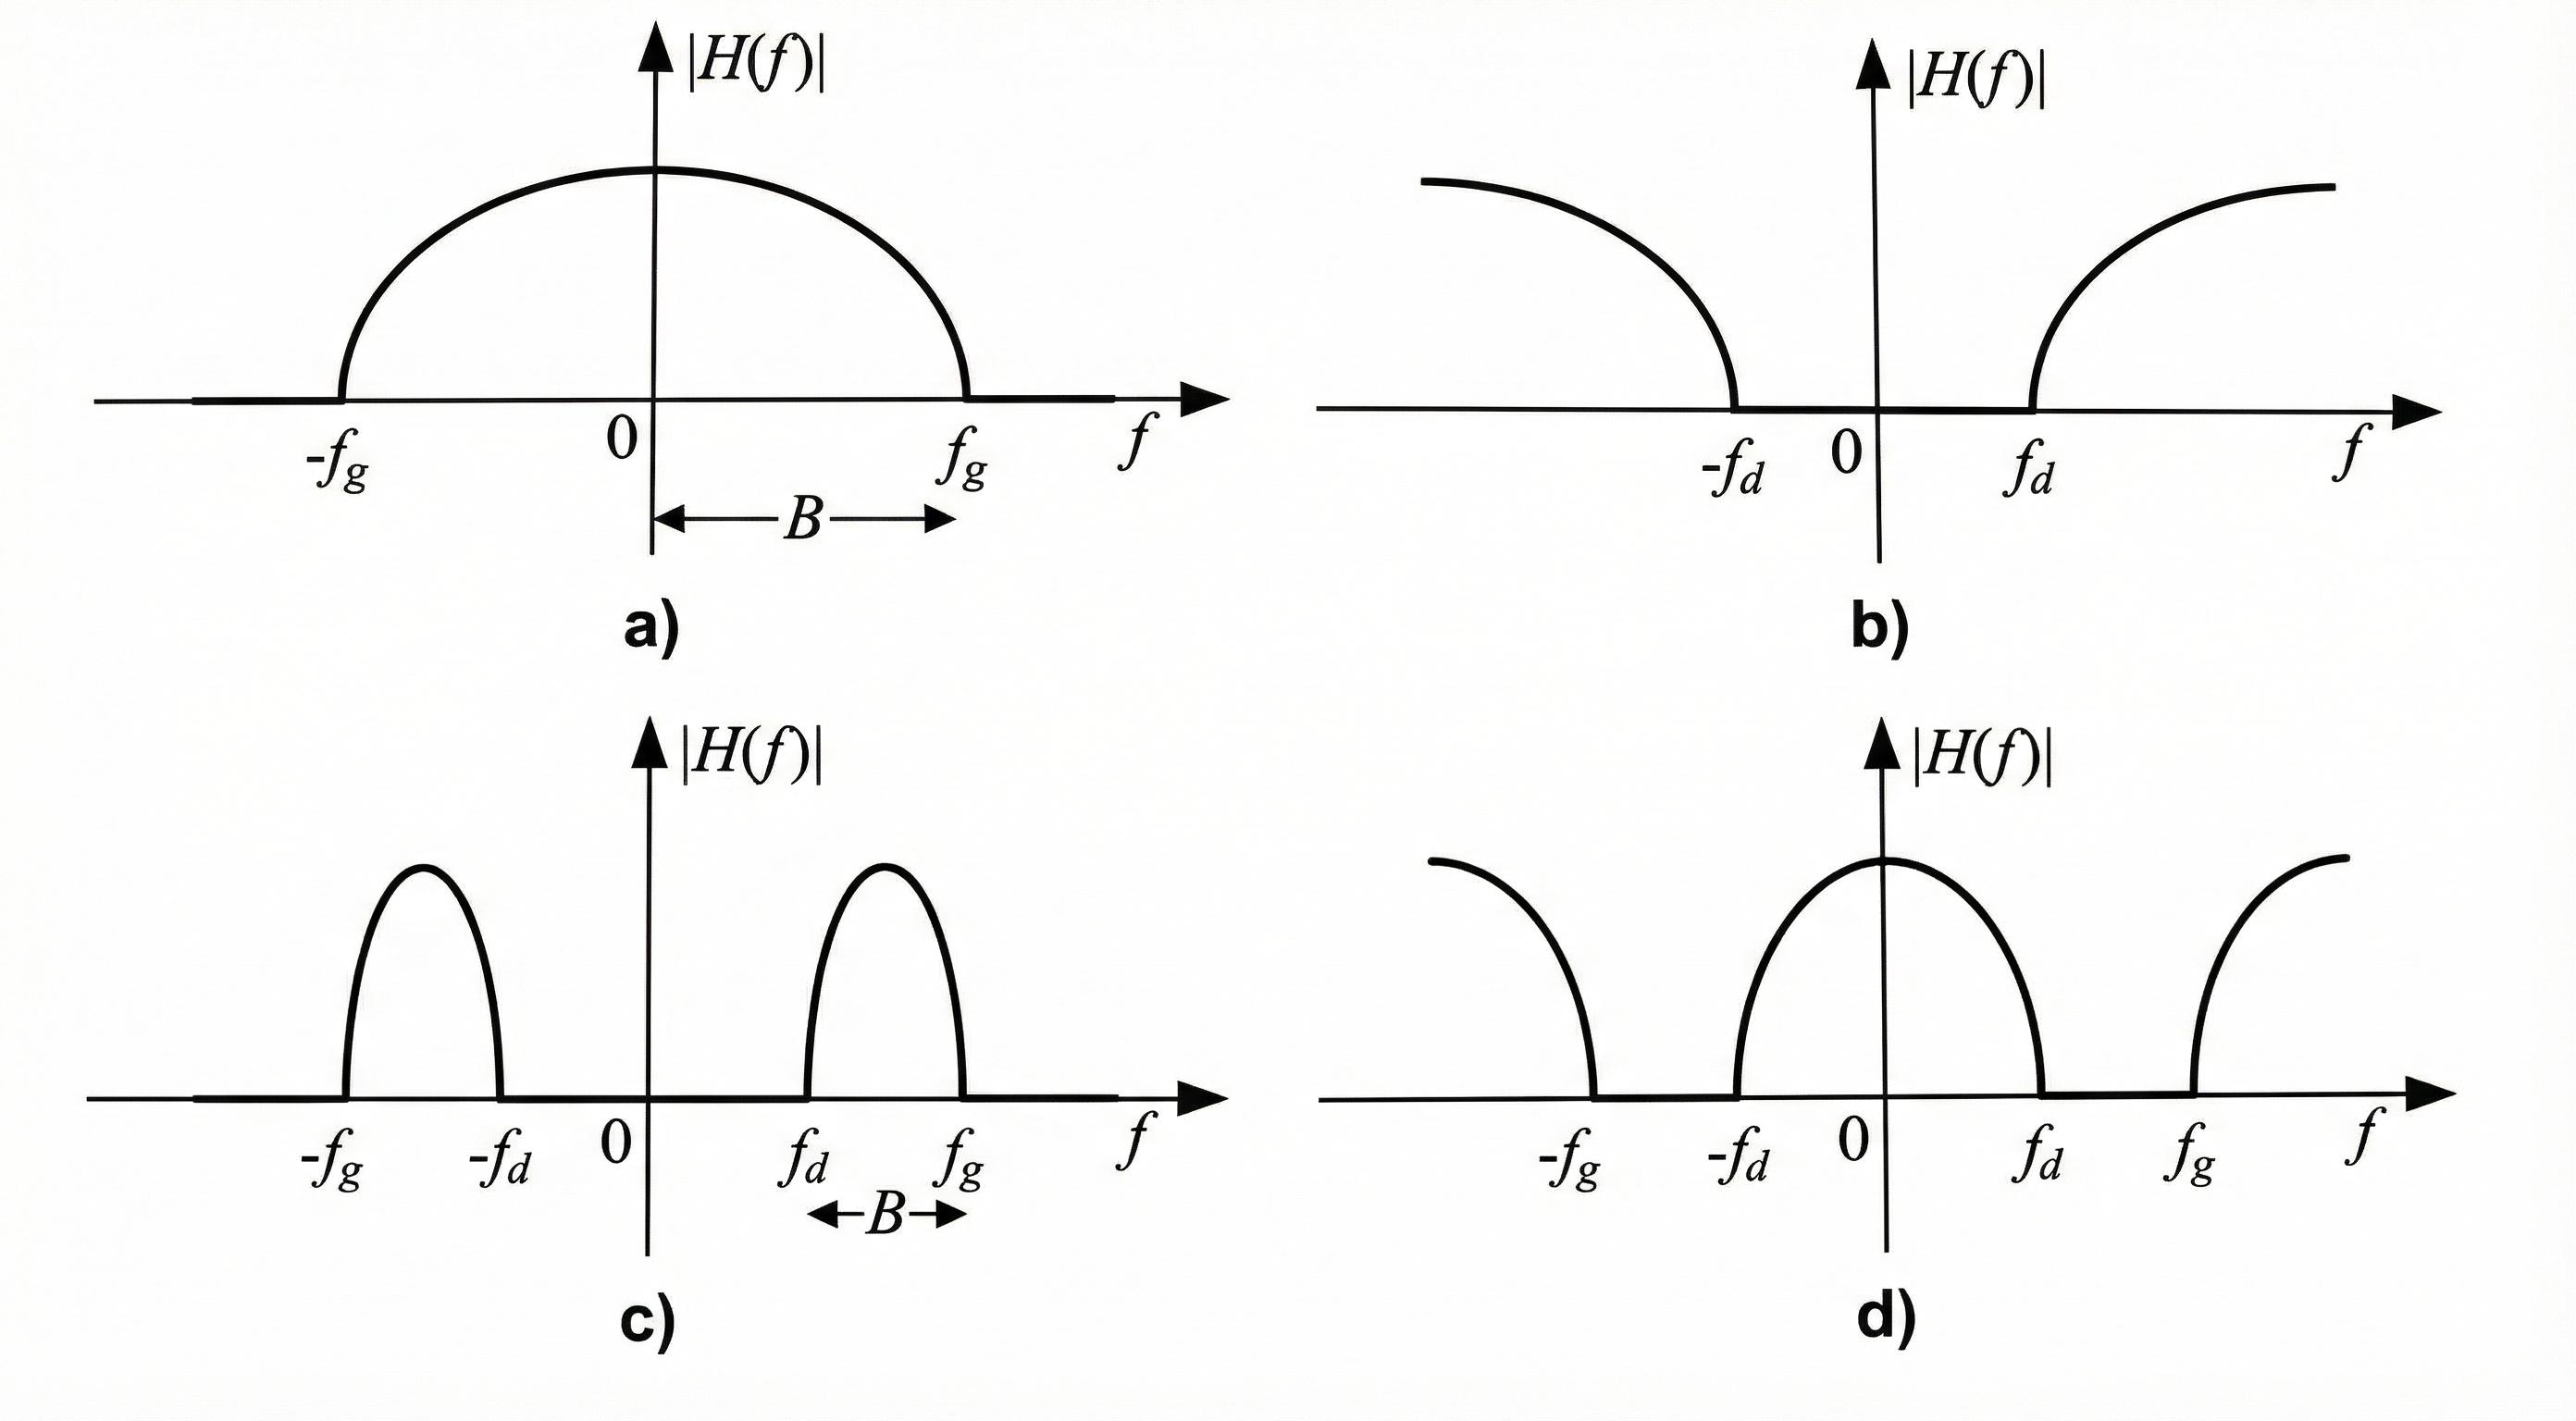
\includegraphics[width=0.5\textwidth]{assets/B.png}
	\end{center}
\end{multicols}
\end{document}

